% Carried over verbatim from monograph/main.tex (Study 1 record, 13 Sep 2026).
\chapter{Exact provenance recovery}\label{s1:ch:ch06_exact_provenance_recovery}

\section{SIPaKMeD Branch A: filename hierarchy}

Branch A parses the released directory and filename convention. For example, \artifact{im_Dyskeratotic/CROPPED/001_03.bmp} maps to parent \artifact{Dyskeratotic/001}. This route is deterministic, fast, and used for the canonical split map. Its weakness is that a parsing bug could produce internally tidy but wrong identifiers. That is why Branch B was required.

\section{SIPaKMeD Branch B: independent content matching}

For crop $x$ and candidate parent region $r$, normalized cross-correlation is
\begin{equation}
\operatorname{NCC}(x,r)=
\frac{\sum_u(x_u-\bar{x})(r_u-\bar{r})}
{\sqrt{\sum_u(x_u-\bar{x})^2}\sqrt{\sum_u(r_u-\bar{r})^2}}.
\end{equation}

Branch B never uses Branch A's parent assignment in the query. It ranks every same-class parent at quarter resolution, refines the five best candidates at full resolution, and records the winning location as a bounding box. A multiscale fallback exists only for unresolved cases. Matching is bounded by class working sets so the complete parent image collection does not have to remain in memory.

\begin{figure}[H]
\centering
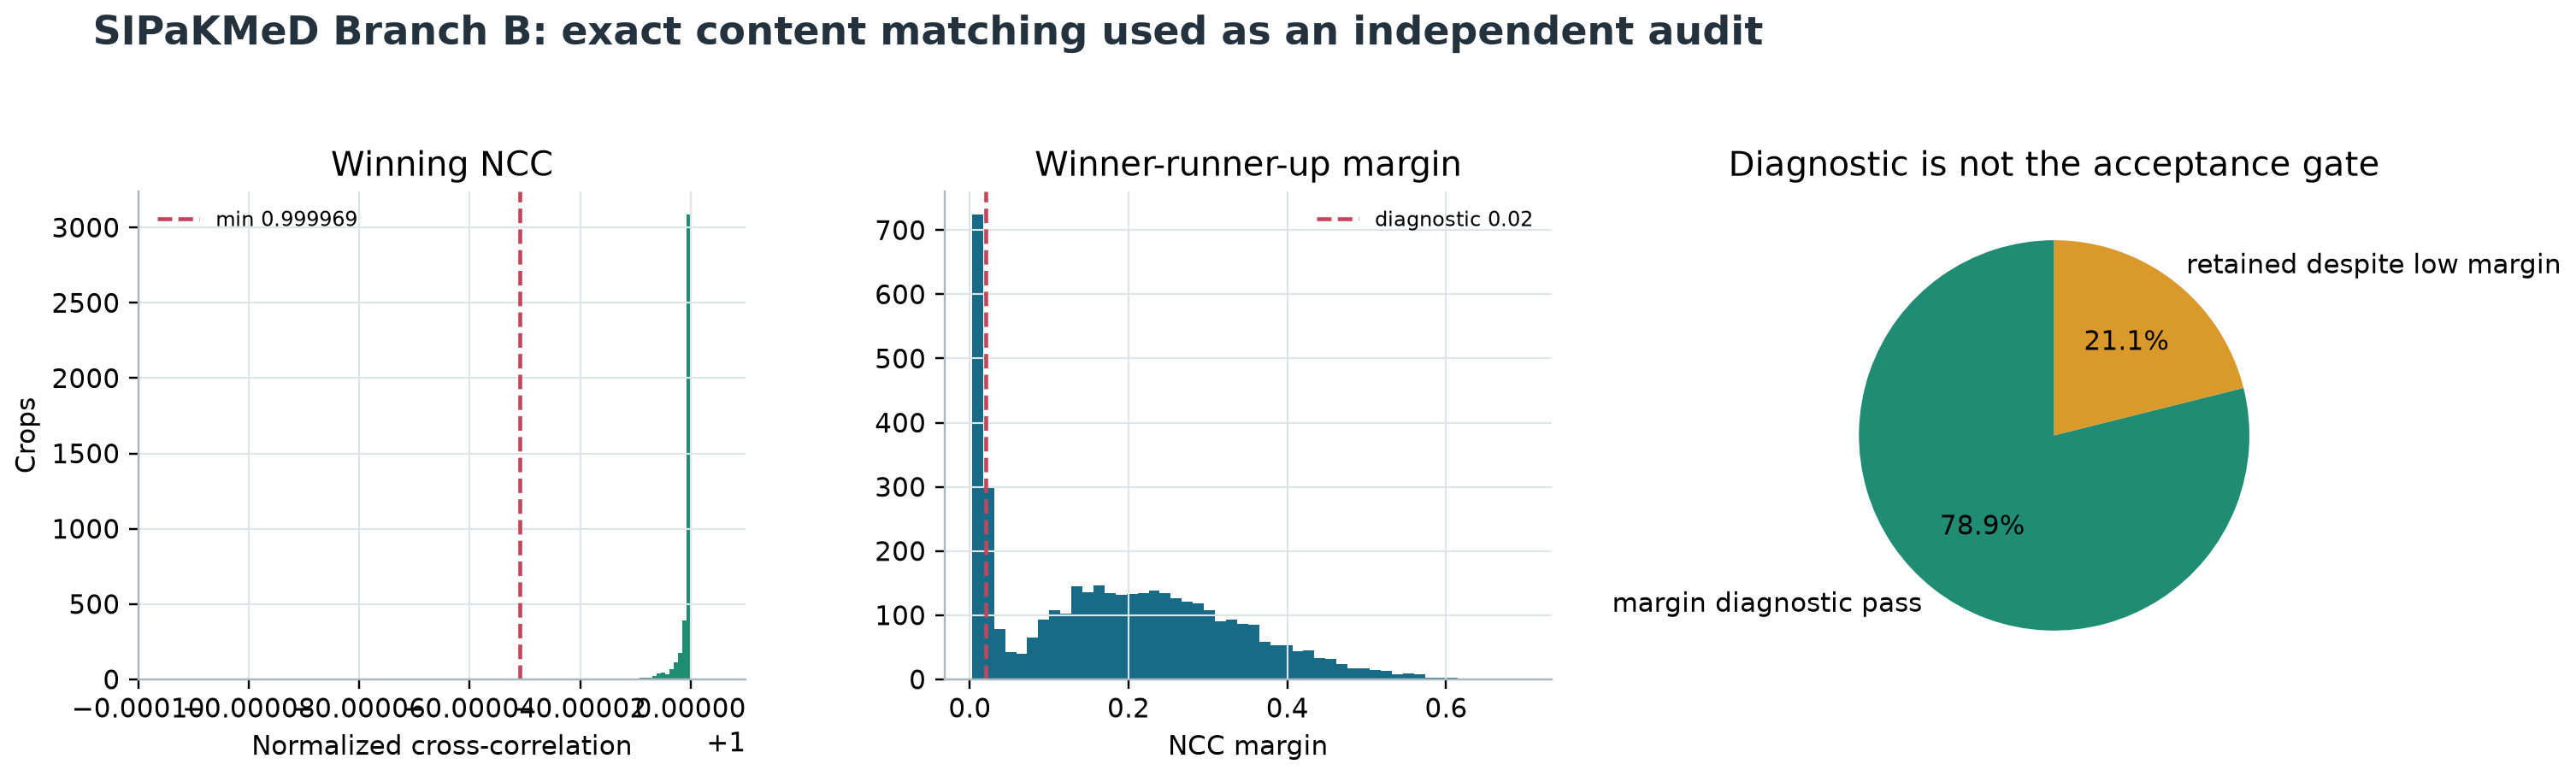
\includegraphics[width=\textwidth]{provenance_diagnostics.png}
\caption{Branch-B diagnostics. The minimum winning NCC is 0.999969. The 0.02 runner-up-margin rule is intentionally only a diagnostic: 3,195 crops pass it and 854 do not, yet all rows agree with Branch A and all boxes remain contained.}
\label{s1:fig:provenance-diagnostics}
\end{figure}

\begin{figure}[H]
\centering
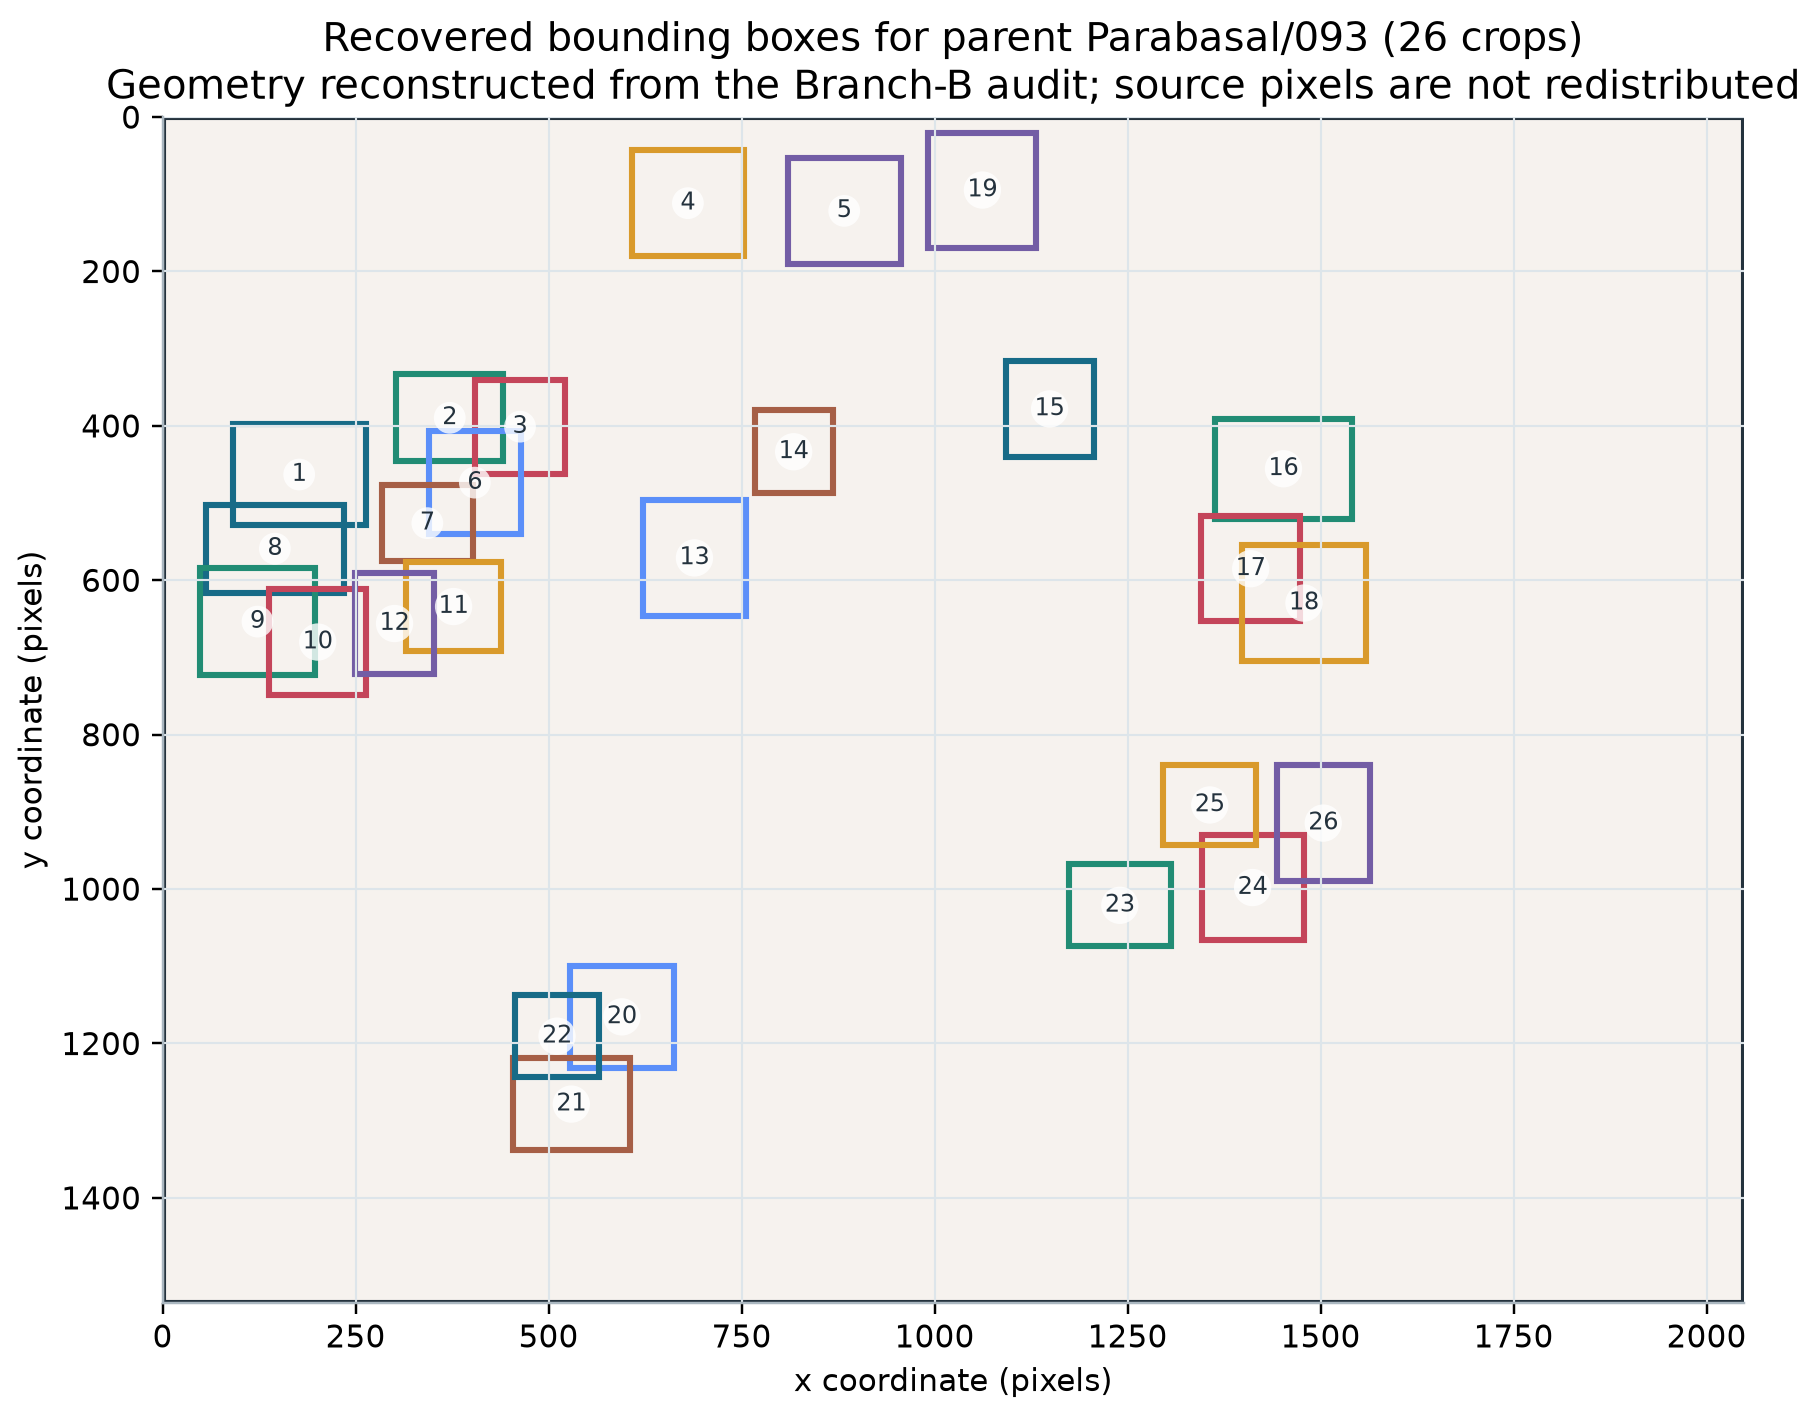
\includegraphics[width=0.77\textwidth]{recovered_bbox_example.png}
\caption{A real recovered-coordinate example for the parent with the largest crop count. Only rectangle geometry is displayed; source pixels are not redistributed. Overlapping rectangles make literal source-pixel sharing possible.}
\label{s1:fig:bboxes}
\end{figure}

\section{Why the auxiliary acceptance flag is false for many correct rows}

The \artifact{accepted} field in Branch B encodes a conservative confidence-plus-margin diagnostic. It is not the registered provenance acceptance outcome. Many microscope fields contain visually repetitive background, so a correct near-perfect winner can have another near-perfect candidate. Substituting this diagnostic for the registered 99\% cross-branch agreement rule would discard 854 correctly mapped crops after looking at an arbitrary margin. The project instead retains every row and exposes the ambiguity measure.

\section{Cx22, CRIC, and Herlev recovery}

Cx22 uses source names and ROI coordinates decoded from the authors' three MATLAB generator releases. Every source resolves against the declared 686-image CCEDD set, and rare edge-touching requested boxes are clipped exactly as the generator code specifies. The released Cx22 archives contain generator metadata and masks rather than a second independent RGB crop array, so an A/B image-content branch cannot be constructed from the public package alone. Applicable checks are source existence, exact metadata decoding, generator geometry, bounds, and subset overlap.

CRIC uses the released classifications table: source-image identity and coordinates directly define the map. Herlev assigns each released cell to itself. Neither route pretends to recover unavailable patient identity.

\section{Verification outcome}

\begin{table}[H]
\centering
\caption{Provenance gates.}
\label{s1:tab:provenance-gates}
\begin{tabularx}{\textwidth}{lrrXl}
\toprule
Dataset & Observations & Parents & Applied evidence & Outcome \\
\midrule
SIPaKMeD & 4,049 & 966 & 4,049/4,049 A/B agreement; 4,049 contained boxes; exact class totals & \pass \\
Cx22 & 1,320 & 514 & generator names/ROIs; 686 sources resolve; 1,320 contained clipped boxes & \pass \\
CRIC & 11,534 & 400 & released source identities and coordinates; no patient-ID claim & \pass \\
Herlev & 917 & 917 & one released cell per parent & \pass \\
\bottomrule
\end{tabularx}
\end{table}

No observation was excluded. The five SIPaKMeD parent counts are exactly 126/108/238/271/223 in corrected release order. All crop counts sum to 4,049.
